A \emph{permutation} is an ordered arrangement of a set of distinct elements. Consider the set $\{1, 2, 3\}$. One possible ordering is \texttt{123}, where the elements appear in their natural order. Another is \texttt{231}, where 2 comes first, followed by 3 and 1. Each such arrangement — where all elements are used exactly once and appear in a specific sequence — is called a permutation of the set.

For a set of size $n$, the total number of such arrangements is given by the factorial function, denoted $n!$. This is because there are $n$ choices for the first position, $n-1$ for the second, and so on, yielding:
\[
n! = n \times (n-1) \times (n-2) \times \cdots \times 2 \times 1.
\]
The number of permutations grows as follows:
\[
1! = 1,\quad 2! = 2,\quad 3! = 6,\quad 4! = 24,\quad 5! = 120,\quad 6! = 720,\quad 7! = 5040.
\]
This rapid — factorial — growth means that although the idea of permutations is elementary, the total number becomes intractable to list or store explicitly even for moderate $n$.

To visualize the implications, suppose one attempts to list all permutations of $\{1, 2, 3\}$: these are \texttt{123}, \texttt{132}, \texttt{213}, \texttt{231}, \texttt{312}, and \texttt{321}. Each permutation has length 3, so listing them end-to-end would yield a string of length $6 \times 3 = 18$. For larger $n$, such direct listings become prohibitively long. Moreover, this naive approach repeats overlapping segments across permutations, introducing redundancy. Understanding and managing this combinatorial explosion is relevant to more questions of encoding, compressing, or other problems in the space of permutations.

A \emph{superpermutation} on $n$ symbols is a finite string that contains, as contiguous substrings, every one of the $n!$ distinct permutations of those symbols. In contrast to merely listing permutations separately, a superpermutation aims to \emph{compress} all of them into a single sequence, reusing overlapping segments wherever possible. The constraint is that each permutation must appear somewhere in the string uninterrupted.

Consider the case $n = 2$. The two permutations of the symbols $\{1, 2\}$ are \texttt{12} and \texttt{21}. A superpermutation must therefore include both \texttt{12} and \texttt{21} as substrings. The shortest such string is \texttt{121}. It contains \texttt{12} starting at position 1 and \texttt{21} starting at position 2. This is the minimal superpermutation for $n = 2$, and it has length 3.

For $n = 3$, there are $3! = 6$ permutations: \texttt{123}, \texttt{132}, \texttt{213}, \texttt{231}, \texttt{312}, and \texttt{321}. One example of a minimal superpermutation that includes all six of these as contiguous substrings is \texttt{123121321}. It has length 9, and each of the six permutations occurs once within it. No shorter string satisfies the same condition.

The central question posed by the \emph{superpermutation problem} is: what is the minimal possible length of such a string for general $n$? That is, given $n$ distinct symbols, what is the shortest string over those symbols that contains every one of their $n!$ permutations as contiguous substrings? As $n$ increases, this problem becomes computationally and combinatorially challenging. The number of permutations grows rapidly, and so does the complexity of arranging them with maximal overlap. The search for minimal superpermutations remains an active area of combinatorial optimization.

At first glance, the problem of constructing a superpermutation may appear manageable. One might attempt a straightforward solution by writing out all $n!$ permutations of the $n$ symbols and concatenating them end-to-end. Since each permutation is of length $n$, this method produces a string of total length $n \cdot n!$. For example, for $n = 3$, this naive approach would yield a string of length $3 \times 6 = 18$. While this guarantees that all permutations are present, it is highly inefficient. Adjacent permutations often share common segments — such as matching suffixes and prefixes — and these overlaps can be exploited to significantly reduce the total length.

The trick is that permutations can be arranged so that the end of one serves as the beginning of the next. For instance, the permutation \texttt{123} ends in \texttt{23}, and \texttt{231} begins with \texttt{23}; by placing them consecutively as \texttt{1231}, the two permutations are both represented, and the shared segment \texttt{23} is not duplicated. This principle of overlap allows one to compress multiple permutations into a single string, hopefully, without repeating identical sequences.

\begin{figure}[ht]
 \centering
 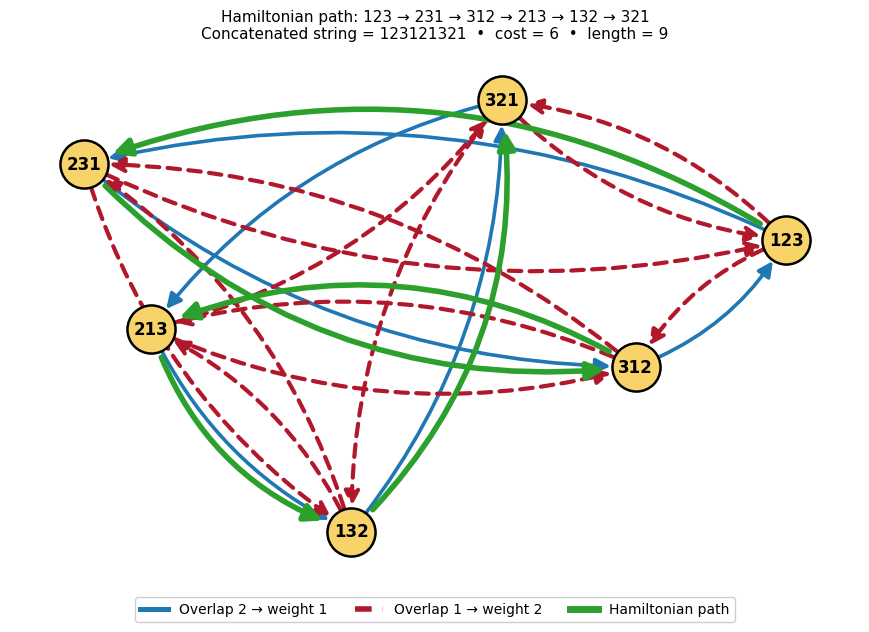
\includegraphics[width=0.7\textwidth]{39_SuperpermutationsBreakthrough/GRAPH2.png}
 \caption{Permutation overlap digraph for $n=3$. Each node is a permutation of $\{1,2,3\}$. A directed edge $A \to B$ exists when a suffix of $A$ matches a prefix of $B$, with \emph{overlap} length $k$. The \emph{weight} is $w = n-k$, i.e.\ the number of extra symbols needed to append $B$ after $A$. Edges with $k=2$ (weight $1$) are shown in solid blue, edges with $k=1$ (weight $2$) in dashed red. The highlighted green path is the Hamiltonian path $123 \to 231 \to 312 \to 213 \to 132 \to 321$, yielding concatenated string $123121321$ of length $9$ and total cost $6$.}
 \label{fig:permgraph3}
\end{figure}

For small values of $n$, exact solutions have been found. Remarkably, for $n = 1$ through $n = 5$, the shortest superpermutations are known, and their lengths follow a simple closed-form pattern:
\[
L(n) = \sum_{k=1}^n k! = 1! + 2! + 3! + \cdots + n!.
\]
For example:
\[
L(3) = 1! + 2! + 3! = 1 + 2 + 6 = 9, \quad
L(4) = 33, \quad
L(5) = 153.
\]
This empirical closed-form suggested a natural conjecture: that the shortest possible superpermutation on $n$ symbols always has length equal to $\sum_{k=1}^n k!$. The conjecture was elegant and aligned with all known cases. For years, no counterexamples were found, and the formula became widely assumed to be correct.

That assumption remained unchallenged until 2014, when it was definitively disproven. A construction was found that produced a superpermutation on six symbols with total length 872 — precisely one character shorter than the conjectured value of
\[
1! + 2! + 3! + 4! + 5! + 6! = 873.
\]
This counterexample showed that the conjectured bound, though valid for $n \leq 5$, does not hold in general.

The origin of this disproof traces back to an unexpected source: an anonymous discussion thread on the imageboard website 4chan. Founded in 2003, 4chan hosts ephemeral user-generated content across numerous boards organized by theme. Messages are anonymous by default, and threads are subject to automatic deletion without archival. The site's culture is informal, transgressive, and often dismissive of academic conventions. One of its boards, labeled \texttt{/sci/}, is nominally dedicated to science and mathematics. Despite inconsistent signal-to-noise, the board occasionally features serious technical inquiry.

In 2011, an anonymous user on the \texttt{/sci/} board of the website 4chan posed a question that, at first glance, seemed whimsical: what is the shortest possible viewing sequence that includes every ordering of the 14 episodes of the anime \emph{The Melancholy of Haruhi Suzumiya}? The show, known for its non-linear narrative and varying episode orders across different broadcasts, had developed a cult following that embraced its combinatorial potential. Beneath the framing, however, lay a precise mathematical question: how short can a string be while still containing every permutation of a 14-element set as a contiguous substring? In effect, the prompt was a popular-culture formulation of the superpermutation problem for $n = 14$.

In response, another anonymous poster provided a compact but mathematically rigorous derivation of a new general lower bound:
$$
L(n) \geq n! + (n - 1)! + (n - 2)! + n - 3
$$

This inequality, valid for all $n \geq 2$, immediately strengthened all previously known bounds. Though presented informally, the proof was ultimately correct. It treated permutations as vertices in a directed graph, with directed edges representing overlaps between adjacent substrings. The minimal-length superpermutation corresponded to a Hamiltonian path through this graph, and the proof established a lower bound on the total cost of any such path by analyzing the unavoidable overlaps.

Despite its correctness and novelty, the result went largely unnoticed at the time. The platform offered no mechanisms for citation or persistence: posts were anonymous, threads expired automatically, and archival relied entirely on user initiative. The derivation was eventually copied to a fandom-hosted mathematics wiki, but remained obscure and disconnected from formal literature.

In 2014, mathematician Robin Houston independently rediscovered the argument, verified its correctness, and recognized its significance. He publicized the result, incorporated it into ongoing research, and cited the unknown author as “Anonymous 4chan Poster” — a designation that remains standard in subsequent academic references. The original poster has never been identified.

The impact was immediate. The new lower bound provided a rigorous floor against which all proposed constructions could be measured. Shortly thereafter, Houston constructed a superpermutation on six symbols of length 872 — one less than the conjectured minimum of 873 — thereby disproving the long-standing sum-of-factorials conjecture. The result showed that minimal lengths could deviate subtly, but definitively, from previous expectations.

In 2018, an accomplished sci-fi author and mathematician Greg Egan proposed a constructive upper bound:
$$
L(n) \leq n! + (n-1)! + (n-2)! + (n-3)! + n - 3
$$

placing the known range for $L(n)$ within a narrow window, bounded, yet not tightly, from above and from below.

The 4chan derivation now stands as a rare episode in modern mathematics: a significant and previously unknown lower bound for a classical problem, derived anonymously, informally posted, largely ignored, and later validated by professionals. It illustrates how insight can originate outside institutional settings, and how easily such insight can be lost when detached from systems of attribution, preservation, and dissemination. Nevertheless, the mathematics holds. The “Haruhi Problem” has since entered the literature as a textbook case in combinatorial optimization — and its solution, at least in part, belongs to a nameless contributor with no affiliation, no traceable authorship, and a correct idea.

\vspace{4em}
\begin{center}
   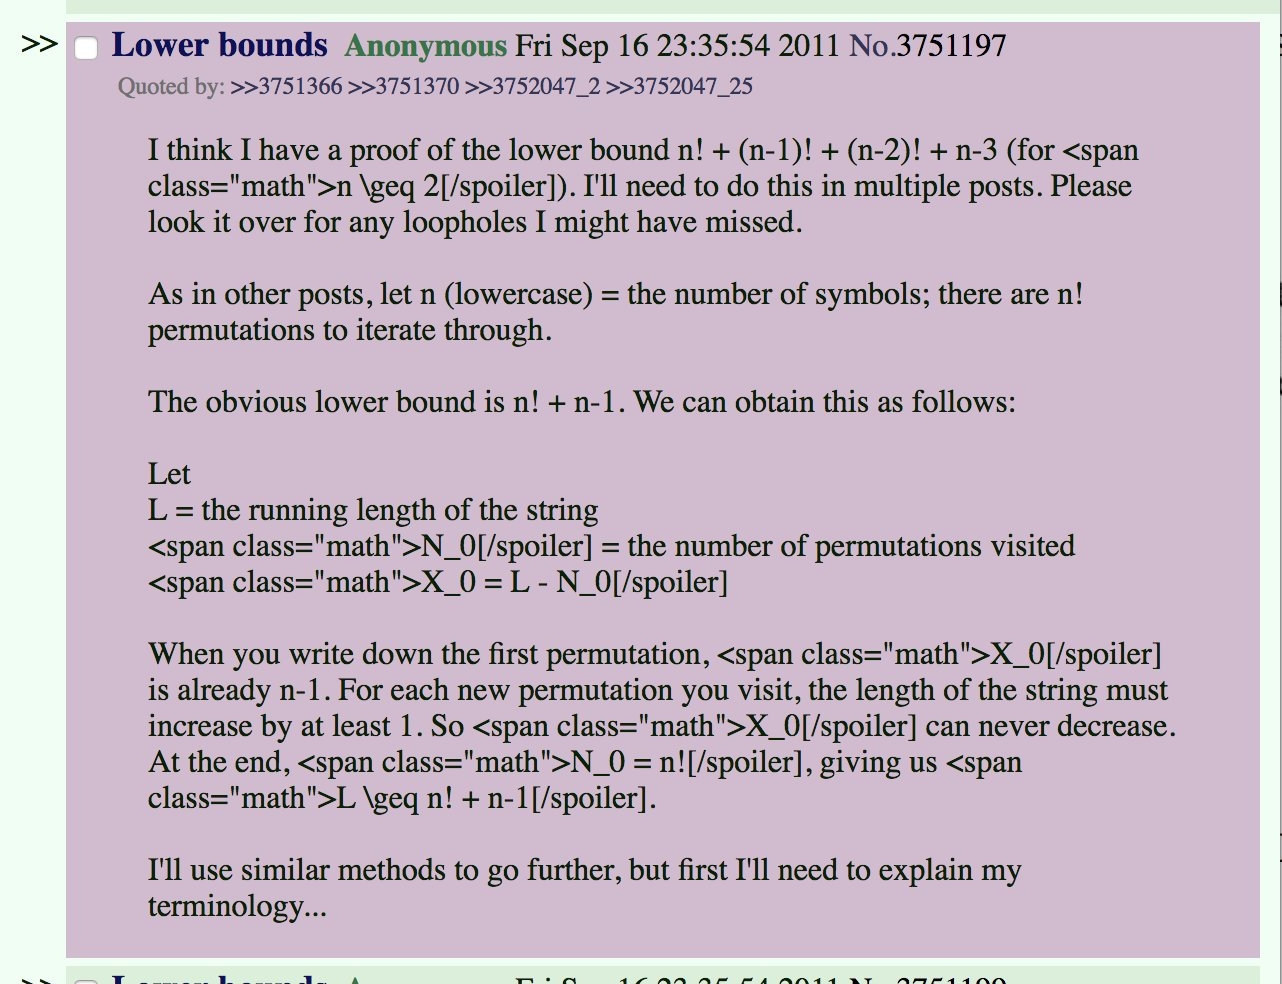
\includegraphics[width=0.8\textwidth]{39_SuperpermutationsBreakthrough/DrTcMa7VYAApwpb.png}\\
   {\small\textit{The original 4chan post}}
\end{center}





